\section[Backgroud on Quantum Metrology]
{Background on Quantum Metrology}
\thiswatermark{\put(1,-241){\color{l-grey}\rule{84pt}{48pt}}
\put(84,-241){\color{grey}\rule{410pt}{48pt}}}


\quotes{Roger J. Barlow}{In the real world, doing real experiments, statistics began to matter}

\vspace{0pt}
\lettrine[lines=2, findent=3pt,nindent=0pt]{I}{n} this chapter we will study the basics of Quantum Metrology, which stands for the science of enhanced metrology by quantum phenomena.
On the other hand, metrology, as the science of measuring, has played an essential role for the development of the technology as we know it today.
It studies several aspects of the estimation process, such as which strategy to follow in order to improve the precision of an estimation or which is the bound for the precision.
Metrology also covers all intermediate process fo the estimation, from the design aspects of a precise measuring device, to the most basic concepts of estimation, which lead at the end to a better understanding of it as a whole.

In this sense, with the discovery of the Quantum Physics and the development of Quantum Mechanics, new doors for advances in metrology were open in the early decades of the 20th century.
First, Quantum Theory embrased the so-called field of Quantum Information, which merges the notions of the theory of information and computer science, among others subfields, with the quantum mechanics.
This new field of Quantum Information is in the basis of Quantum Metrology.
Moreover, those emerging fields rapidly became into very interesting interdisciplinary playgrounds of science attracting the interest of many scientists as well as resources for their researches.
Just to menetion that the role of the so-called entanglement, an exclusive feature of Quantum Mechanics which cannot be completelly described using classical probabilistic theories, is essential in this context.
With the aim of completelly understand this concepts, many scientists world wide have integrated their efforts.
Said this, the entanglement also is in the center of theoretical concepts in Quantum Metrology.
In the Quantum Metrology framework, we will focus on the achievable precision of the systems.
We will show as well different strategies to achieve the desired results.

On the other hand, a very important field of science must be highlighted by its own meriths.
We are mentioning the statistics, without which many descriptions of the actual and past physical findings would lack of the rigorous interpretation needed for the complexity of data samples.
It basically helps to analyse raw data to find special properties out of it.

\subsection{Background on statistics and the theory of estimation}

In this section, we will enumerate the basic concepts of statistics as well as the estimation process.
As we said, the main mathematical tools used by the metrology science belong to statistics.
Moreover, we are expecially interested in estimation theory.
The statistics main characteristic is that it makes the raw data under consideration comprehensible from the human perspective.
The data can be anything, from a set of different heights of a basketball team, to the outcomes of a coin toss, or the wavelength of photons coming out of some sample.
The aim of this section is to give the reader sufficient material to follow this thesis and make it comprehensible from the beginning\footnote{
For a more detailed material, check statistics book as weel as mathematics book for scientist and engeneers \citep{Riley1998, BarlowXXXX}}.

\subsubsection{Probability, data samples, average and variance}

The probability indicates the relative chance of an event to happen.
For instance, if there is a box with ten red balls and five blue balls, considering that the balls of the same color are indistinguishable and that we extract one randomly, we have $\frac{5}{10+5}=\frac{1}{3}$ of probability to obtain a blue ball and $\frac{2}{3}$ to obtain a red ball.
The reader may notice many properties a probability should have, such as that the probability of any event to happen is always one or that a probability is always given by a number in between zero and one.
For more details, there are many interesting textbooks or chapters of some textbook about Probability Theory one could follow if interested.
The following References~\citep{Riley1998, BarlowXXXX} are some of those books.

When someone has a data sample at hand, it might come from diverse sources and might be represented using multiple forms such as numbers or words (for instace, a table of names of people), the first thing one tries to accomplish is to analyse the data to extract the relevant properties from it.
A data sample always come from a population sample, i.e., the data sample might not be complete (one could lose some in the process) neither exact (a measuring device always have an error when estimating a magnitude).
Hence, the data sample comes attached with a probability for each data element.
In the subsecuent paragraphs, we will describe this relation and we will enumenrate the most useful properties and formulas for the comprehensions of this thesis.

First of all, we will explain our notation which follows the one used on Reference~\citep{Riley1998}.
A probability function gives the probability of an event $x$ to happen when measuring some random variable $X$, and it is denoted by $\prob(X=x)$.
Second, the $N$ elements of a data sample are considered to come from $N$ random variables with the corresponding $N$ values due to the random nature of the measuring, $\{X_i=x_i\}_{i=1}^N$.
The joint probability of those random variables is in general not separable.
This is due to the fact that the outcomes could depend on the rest of the outcomes or some other more complex relation that makes the most general case to be non-separable from the probabilistic point of view.
Therefore we define this PDF as an $N$ variable function
\be
  \prob(\bs{X}=\bs{x}) \equiv \prob(X_1=x_1,X_2=x_2,\dots,X_N=x_N).
\ee
If separable this is written by
\be
  \prob(\bs{X}=\bs{x}) = \prod_{i=1}^N\prob(X_i=x_i)
\ee
and it is the case for many relevan cases.

When some property of the system is defined as a function of random variables, the result is also a random variable with another transformed PDF.
For example, we measure the position of a body at some moment.
If the system was at rest on the origin at initial time and the acceleration is known to be constant, then from the position one can infeer on the value of the acceleration by using $A=2X/t^2$, where $X$ denotes the position at intant $t$ and $A$ the acceleration.
If $X$ is a random variable, which is the general case when measuring the position of a body, then the probability is computed in this case by
\be
  \prob(A=a) = \frac{\text{d}x}{\text{d}a}\prob(X=x)=\frac{2}{t^2}\prob(X=x).
\ee
In general for the multiple random variable case transformations, we must require that
\be
  |\prob(\bs{X}=\bs{x})\,\text{d}x_1\text{d}x_2\dots\text{d}x_N|=|\prob(\bs{Y}=\bs{y})\,\text{d}y_1\text{d}y_2\dots\text{d}y_N|.
\ee
This leads to some interesting formulas we will discuss later.

We now stick to the simplest case on which the data is a collection of values of the same random variable describing the same physical one-dimensional data population.
Some definitions reasonable to mention in this thesis arise for those kind of data samples: the average, variance, moments and central moments.
The arithmetic average (there are other types of average one can find in the textbooks) is computed by
\be
  \overline{x}=\frac{1}{N}\sum x_i.
\ee
The variance is related with the spread of the data and computed by
\be
  \sigma^2=\frac{1}{N}\sum (x_i-\overline{x})^2,
\ee
where $\sigma$ is the standard deviation.
Different moments are computed by $\overline{x^r}=\frac{1}{N}\sum x_i^r$ while central moments are of the form of $n_r=\frac{1}{N}\sum (x_i-\overline{x})^r$.
Notice that the variance is the second central moment of the data sample.
For completeness, when each element of the data consists of more than a number, e.g., $(x_i,y_i,z_i)$, the covariance between two data kinds, in the following case $X$ and $Y$, is obtained by
\be
  V_{X,Y} = \frac{1}{N}\sum_{i=1}^N (x_i-\overline{x})(y_i-\overline{y}).
\ee

Those functions also apply to the probability distribution functions.
While these last ones may be unkown functions for us, as soon as we collect all the possible data or we are in the large number regime the variances of the data sample and of the data population, the means, the covariances and so on so forth, they must coincide.
We will try to keep this distinghusion as clear as possible.
In general the mean values of any function over data sample values $g(x)$ are denoted with a bar over a lowercase variable, e.g., $\overline{x^r}$ for the $r$-th moment, while the mean values of any function applied to the data population $g(X)$ is written following some textbooks by $\text{E}[g(X)]$.
One clearlly may distinguish two cases here: one for continuous functions where the expectation values or the means are computed integrating over all the posible values, and the other case on which $\prob(\bs{X}=\bs{x})$ can take only discrete values.
For completeness here are the two definitions
\be
  \text{E}[g(\bs{X})] = \lcor
  \begin{split}
    &\int g(\bs{x}) \prob(\bs{X}=\bs{x})\,\text{d}^N \bs{x},\\
    &\sum_{i,j,\dots} g(\bs{x}) \prob(\bs{X}=\bs{x}).
  \end{split}
  \right.
\ee
One more deffinition needs our attention and it is the variance any function $g(X)$ denoted by $\text{V}[g(X)] \equiv \text{E}[g(X)^2] - E[g(X)]^2$.

\subsubsection{Frecuentist vs. bayesian approach}

\subsubsection{Estimators and Fisher information}

Let us supose that the data sample has encoded some wanted parameters $\bs{a}\equiv(a_1,a_2,\dots)$.
The underlying probability, in general also unknown, may be conditioned by the real values of the wanted parameters $\bs{a}$.
The probability of the data sample is therefore writen as
\be
  \prob(\bs{X}=\bs{x}|\bs{a}),
\ee
where "$|\bs{a}$" indicates its dependency on these parameters.
At this point, notice that an estimate of the the wanted parameter based on the data sample has the form of a function the random variables.
Therefore as mentioned before, an estimator of $a$, which is how is called this quantity and is denoted by $\hat{a}$, is another random variable with a PDF of the form of
\be
  \prob(\hat{a}|\bs{a})\,\text{d}\hat{a} = \prob(\bs{X}=\bs{x}|\bs{a})\,\text{d}x_1\text{d}x_2\dots\text{d}x_N.
\ee
For short, we omit on writing $\bs{X}$ from now on, thus the conditional joint pobrability of $N$ random variables is written as $\prob(\bs{x}|\bs{a})$.

As we said, an estimator is defined to be a function of the data sample.
For example, one of such estimators is the estimator of the mean value of the data population, in general unknown.
The mean value of the data population, which in general we do not have acces to, is denoted usually by $\mu$.
Notice that $\mu$ is in general different from the mean value of the data sample $\overline{x}$.
A valid estimator for the population mean value would be the arithmetic mean of the data sample, i.e., $\hat{\mu}=\overline{x}$.

An important notion of an estimator is its \emph{efficiency}, i.e., whether it has smaller variance than another.
The more efficient estimator the smaller variance it has.
Remember than an estimator is a random variable so it must have a variance that comes from the data population, i.e., from $\prob(\hat{a}|\bs{a})$ in this case.

For an estimator of any kind there is a theoretical lower bound for its variance.
For the proof of the previous observation, which we compute for continuous random variables without lossing of generality, we start with the normalisation of the PDF
\be
  \int \prob(\bs{x}|\bs{a})\,\text{d}^N\bs{x} = 1.
\ee
Next, we compute the partial derivate over $a$ such that
\be
  \int \partial_a\prob(\bs{x}|\bs{a})\,\text{d}^N\bs{x} = \int \partial_a\big(\ln  \prob(\bs{x}|\bs{a})\big) \prob(\bs{x}|\bs{a}) \,\text{d}^N\bs{x} = 0,
\ee
where for simplification, we ommit the arguments of the joint probability on the second equality.
From Eq.~\eqref{}, it turns out that the Eq.~\eqref{} is the expectation value of $\partial_a(\ln\prob)$.
Finally if we have an unbiashed estimator, for which the true value $a$ coincides with the expectation value of the estimator $\text{E}[\hat{a}]$, its partial differenciation over $a$ must be equal to one,
\begin{align}
  \partial_a\text{E}[\hat{a}] &= \partial_a a = 1, \\
  \begin{split}
    1 &= \partial_a \int \hat{a} \prob(\bs{x}|\bs{a})\,\text{d}^N\bs{x} \\
      &=  \int \hat{a} \partial_a\prob(\bs{x}|\bs{a})\,\text{d}^N\bs{x} =  \int \hat{a} \partial_a\big(\ln  \prob(\bs{x}|\bs{a})\big) \prob(\bs{x}|\bs{a}) \,\text{d}^N\bs{x},
  \end{split}
\end{align}
where we apply the definition of the expectation value of the estimator $\hat{a}$ for continuous variables and we apply as well similar identities as in Eq.~\eqref{}.

At this point we invoke the Schwarz inequallity for two real multidimensional functions $g(\bs{x})$ and $h(\bs{x})$ such that $(\int g h \,\text{d}^N\bs{x})^2\leq (\int g^2 \,\text{d}^N\bs{x}) (\int h^2 \,\text{d}^N\bs{x})$.
With this we can follow the following receipe to obtain a lower bound for the variance of a general estimator.
First the deffinition of the variance looks like
\be
  V[\hat{a}] = E[(\hat{a}-a)^2] = \int (\hat{a} - a)^2\prob(\bs{x}|\bs{a})\,\text{d}^N\bs{x}.
\ee
Second, from Eqs.~\eqref{,} holds that
\be
  \int (\hat{a}-a)\partial_a\big(\ln  \prob(\bs{x}|\bs{a})\big) \prob(\bs{x}|\bs{a})\,\text{d}^N\bs{x} = 1
\ee
because $a$ is not a function of $\bs{x}$.
Hence, using the Schwarz inequality we can write
\be
  \text{V}[\hat{a}] = \int (\hat{a} - a)^2\prob(\bs{x}|\bs{a})\,\text{d}^N\bs{x} \geq \frac{1}{\int \lcua\partial_a\big(\ln \prob (\bs{x}|\bs{a}) \big)\rcua^2 \prob (\bs{x}|\bs{a})\,\text{d}^N\bs{x}},
\ee
which is also known as the Cramer-Rao bound or the Fisher inequality.

With this review on the interesting features of "classical" metrology, we conclude this section.
In the next section, we recall some properties of the Quantum Mechanics and we subsecuentelly follow with the basis of Quantum Metrology. 




\subsection{Quantum Mechanics from metrology perspective}

The ubiquitous probabilistic nature of quantum mechanics forces all the community to know some basics on probability and statistics.

\subsubsection{The quantum state, multi-particle state, entanglement}

A \emph{system state} in Quantum Mechanics lives on a Hilbert space, $\mathcal{H}$.
The system state, $\rho$, has the following properties:
\begin{enumerate}
  \item
  It is Hermitian, so it is invariant under the complex transposition, $\rho=\rho^\dagger$.
  \item Its trace is equal to one, $\tr(\rho)=1$.
  \item It is positive semi-definite, i.e, all its eigenvalues are bigger or equal to zero, $\rho=\sum_{\lambda}p_\lambda \Pi_\lambda$\footnote{
    $\rho=\sum_{\lambda}p_\lambda \Pi_{\lambda}$ is the eigen-representation of the state, where $\Pi_{\lambda}$ are the eigenstates defined on $\mathcal{H}$ too.
    They are as many as the dimension, $d$, of the Hilbert space.
    They are orthonormal under the product defined on such Hilbert space $\mathcal{H}$, i.e, $\tr(\Pi_{\lambda}\Pi_{\lambda'})=\delta_{\lambda,\lambda'}$.
    Nevertheless, there is a extended discussion when Hilbert space is defined for continuous variables, see [XXX].
  } where $p_\lambda\geq 0$ are the scalar eigenvalues.
  It follows that $\sum_\lambda p_\lambda = 1$.
  \item If all $p_\lambda$ are zero except one, the state is a pure state, $\rho=\Pi_\lambda$.
  \item It follows that the quantum states form a convex set where the extremal points are pure states.
\end{enumerate}


The composite system of $N$ different parties lives on $\mathcal{H} = \mathcal{H}^{(1)}\otimes\mathcal{H}^{(2)}\otimes\cdots\otimes\mathcal{H}^{(N)}$ or for short $\mathcal{H} = \bigotimes_{i=1}^N\mathcal{H}^{(i)}$, where $\otimes$ stands for a tensor product like construction.
For instance, this composite Hilbert space could be used to represent a many-particle system, in this case $N$ particles.
A \emph{separable} state on this Hilbert space can be described in the following way,
\be
  \rho = \sum_{i}p_i\rho_i^{(1)}\otimes\rho_i^{(2)}\otimes\cdots\otimes\rho_i^{(N)},
\ee
where $p_i$ are convex weights that sum to one and are equal or bigger than zero.
If not the state is said to be \emph{entangled}.


Angular momentum operators.
The angular momentum algebra comes

Entanglement cannot be described classically.

Evolution

Unitary evolution

Markov

Limblad

Measurements (POVM)

Quantum Information

\subsection{Quantum Metrology}

The evolution of a quantum state can be used to infer on some hidden parameter.
The estimation theory applied to the intrinsic statistical nature of a quantum states has lead to the the formulation of Quantum Metrology as an important subfield.
Merging the probabilistic features of quantum mechanics and the estimation theory is not trivial.
Nevertheless, starting from the pioneering works of Wotters, Braunstein and some other I probably forgot to mention [XXX] were the statistical distance of neighbor states is studied we have lead to amazing results which today drive many experiments and technology.
From the works of Giovannetti et al and Paris on the middle of the last decade fundamental concepts arose, for example the figure of merit quantum Fisher information or the Heisenberg limit.
In this section we will highlight the most important aspects of this field and with this we will conclude this introductory chapter.

The error propagation formula for an estimation of $\Theta$ based on the observable $O$.
\be
  (\Delta \Theta)^2 \geq \frac{\varian{O}}{|\partial_{\Theta}\expect{O}|^2}
\ee

\subsubsection{Quantum Magnetometry}
\label{sec:bg-quantum-metro}

One of the most basic tasks of Quantum Metrology is to address the precision of estimating the magnetic field strength, namely $B$, of an unknown external magnetic field.
In this section we will assume that the magnetic field is homogeneous on the position space.
To consider more advanced situations on which the magnetic field changes linearly with the position, see chapter [XXX].
With the aim of estimating the strength of the magnetic field, a prove state is used in order to interact with it, coupling the magnetic moment of the state and the field itself.
After some time, the state has evolved.
Finally, measuring how the state has changed one would be able to infer on the strength of the magnetic field, basically proportional to the change on the state.

In general, we will say that the magnetic moments of the states come exclusively from the spin angular momentum, neglecting any possible contribution from the orbital angular momentum.
This way the physics is simpler.
This is justified in the sense that most of the recent experiments on this context have been carried out with ion-traps, BECs or at most cold atomic ensembles, which have indeed a negligible orbital angular momentum.

Beside this considerations, the interaction Hamiltonian can be written as,
\be
  H = - \bs{\mu} \cdot \bs{B}
\ee
up to some constant factor.
Now in the simplest case we will choose the magnetic field to be pointing to some fixed direction, for instance, the $z$-direction.
So the magnetic field vector can be written as ${B}=B\bs{k}$, where $\bs{k}$ is the unitary vector pointing to the $z$-direction.
This way estimation problem is much more simple, since one has not to determine the direction of the magnetic field.

The magnetic moment of the system is proportional to the spin angular momentum, $\bs{\mu}=-\mu_\text{B} g_{\text{s}}\hbar^{-1} \bs{J}$, where $\mu_{\text{B}}$ and $g_{\text{s}}$ are the Bohr magneton and anomalous gyromagnetic factor respectively.
Finally, one can rewrite the interaction Hamiltonian as,
\be
  H = \gamma B J_z
\ee
where $\gamma = \mu_\text{B} g_{\text{s}}\hbar^{-1}$ and we have used the fact that $\bs{J}\cdot\bs{k}=J_z$.
Finally, the unitary operator leading the evolution of the system can be written as,
\be
  U = \exp(-i\Theta J_z),
\ee
where the magnetic field strength is encoded into the variable $\Theta=-\mu_\text{B} g_\text{s} t B/\hbar$.
Here $\mu_\text{B}$ stand for the Magneton of Bhor and $g_\text{s}$ for the giro-magnetic constant for the spin angular momentum, and $t$ is the time spent on the evolution.

\begin{figure}
  \centering
  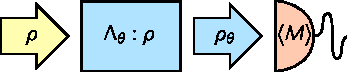
\includegraphics[scale=.85]{img/BG_preparation_encoding_estimation.pdf}
  \caption[Quantum Metrology estimation process]{Secuence of the different steps for the basics of the estimation process on Quantum Metrology. First, an input state $\rho$ enters the region on which the unknown parameter $\Theta$ is imprinted on it, for the most general case, representented with $\Lambda_{\Theta}$. Last, the state that has encoded the parameter $\Theta$ on it is measured and $\Theta$ must be infered from the measured quantity $\expect{M}$.}
  \label{fig:bg-preparation-encoding-estimation}
\end{figure}

\begin{figure}
  \centering
  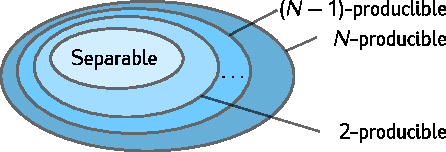
\includegraphics[scale=.85]{img/BG_separability_k_producibility_circle.pdf}
  \caption[Diagram for $k$-producibility sets]{}
  \label{fig:bg-separability-k-producibility-circle}
\end{figure}

\be
  \label{eq:bg-pezze-bound}
  \qfi[\rho,J_z] \geq \frac{\expect{J_y}^2}{\varian{J_x}}
\ee
